\documentclass[conference]{IEEEtran}
\IEEEoverridecommandlockouts
% The preceding line is only needed to identify funding in the first footnote. If that is unneeded, please comment it out.
\usepackage{url}
\usepackage{cite}
\usepackage{amsmath,amssymb,amsfonts}
\usepackage{tabularx,booktabs}
\renewcommand{\arraystretch}{1.4}
\usepackage{algorithmic}
\usepackage{graphicx}
\usepackage{textcomp}
\usepackage[ngerman]{babel}
\usepackage{xcolor}
\def\BibTeX{{\rm B\kern-.05em{\sc i\kern-.025em b}\kern-.08em
    T\kern-.1667em\lower.7ex\hbox{E}\kern-.125emX}}
\begin{document}

\title{MedPlanner\\
{\large Web-Anwendungsentwicklung Sommersemester 2021}
}

\author{\IEEEauthorblockN{Egidia Cenko}
\IEEEauthorblockA{\textit{Medieninformatik} \\
e.cenko@oth-aw.de}
\and
\IEEEauthorblockN{Madina Kamalova}
\IEEEauthorblockA{\textit{Medieninformatik} \\
m.kamalova@oth-aw.de}
\and
\IEEEauthorblockN{Matthias Schön}
\IEEEauthorblockA{\textit{Medieninformatik} \\
m.schoen@oth-aw.de}
\and
\IEEEauthorblockN{Christoph Schuster}
\IEEEauthorblockA{\textit{Medieninformatik} \\
	c.schuster1@oth-aw.de}
\and
\IEEEauthorblockN{Andrei Trukhin}
\IEEEauthorblockA{\textit{Medieninformatik} \\
	a.trukhin@oth-aw.de}
}

\maketitle

\begin{abstract}
Beschreibung der Software-Architektur für das Projekt \textit{MedPlanner} von Team Grün. Dabei wird zunächst allgemein ein Überblick über das System gegeben, Architekturentscheidungen beschrieben und auf Probleme bei der Realisierung eingegangen. Zuletzt wird in Form eines Ausblicks aufgezeigt, wie die Web-Anwendung in Zukunft ausgebaut werden kann.
\end{abstract}

%\begin{IEEEkeywords}
%TODO oder ganz weg 
%\end{IEEEkeywords}


%\section{Aufgabenstellung}
\section{Überblick}
\subsection{Mission Statement}
MedPlanner bietet die Möglichkeit, ärztliche Termine übersichtlich zu verwalten. Es handelt sich hierbei um eine Web-Anwendung, die gezielt auf das Selbstmanagement von Arztterminen abgestimmt ist. MedPlanner ist auf verschiedenen Geräten, einschließlich Computern, Smartphones und Tablets verfügbar. Mithilfe von MedPlanner können zukünftige Arzttermine eingetragen und geplant werden. Es ist vor allem für Privatpersonen gedacht, welche somit einen Überblick über die Vielzahl ärztlicher Untersuchungen behalten können.\\
Zu den wesentlichen Features gehört die Eintragung von Terminen, die man zusätzlich mit Notizen und Tags versehen kann. Weiterhin ist es möglich, Kontaktinformationen für die eigenen Ärzte abzuspeichern. So sind die von MedPlanner gebotenen Kontaktinformationen, wie zum Beispiel Telefonnummer, Adresse und, falls vorhanden, die Webseite der Arztpraxis abzurufen, ohne extra vor einer Terminvereinbarung wiederholt nach den nötigen Informationen zu suchen. MedPlanner bietet außerdem die Funktion Erinnerungs-Mails für vereinbarte Termine zu erhalten. So bekommt der Patient direkt nach Termineintragung in der Web-Anwendung eine EMail-Benachrichtung mit den wichtigsten Informationen zum Arzttermin.


\subsection{Architekturziele}
\begin{table}[!h]
	%TODO remove caption Tabelle1
	\caption{Qualitätsanforderungen}
	\begin{tabularx}{\columnwidth}{>{\bfseries}l|p{57mm}}
		\toprule
		\textbf{Ziel} & Erklärung\\
		\midrule
		Benutzbarkeit & Intuitive Bedienbarkeit und schnelle Erlernbarkeit\\
		Sicherheit & Inhalte sind vor unberechtigtem Zugriff geschützt\\
		Wartbarkeit & Leichte Erweiterbarkeit und Änderung\\
		Leicht zu betreiben & Die Anwendung kann ohne größere Anpassungen genutzt werden\\
		\bottomrule
	\end{tabularx}
\end{table}

\subsection{Kontextabgrenzung}
Die folgende Darstellung visualisiert das zu beschreibende System als Blackbox und zeigt so die Interaktion mit Benutzern und Fremdsystemen auf.
\begin{figure}[!h]
	\centering
	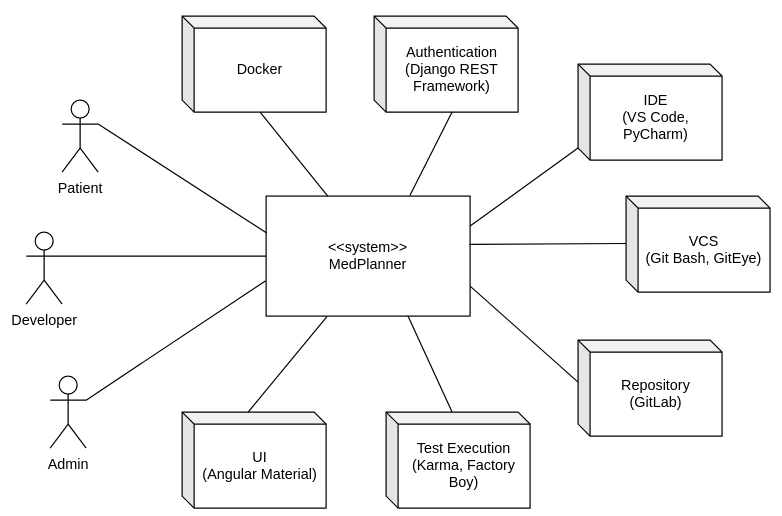
\includegraphics[width=0.9\columnwidth]{./figures/system_context_medplanner}
	\caption{Systemkontext für MedPlanner}
\end{figure}

Menschlicher Akteur ist neben dem Entwickler der Web-Anwendung auch der Admin, der u.a. Daten in die Datenbank einfügen kann, die den Patienten zur Verfügung stehen, wie z.B. die Fachrichtung von Ärzten. Der Patient ist hierbei der eigentliche Nutzer der Web-Anwendung, der eigene Termine und Ärzte einfügen kann. Als externe Systeme gelten neben der Entwicklung und Versionsverwaltung auch weitere Systeme zur Realisierung der Web-Anwendung, z.B. wird für das User Interface \textit{Angular Material} eingesetzt, welches Design-Komponenten bereitstellt. Für die Erstellung von Tests wird im Frontend \textit{Karma} und im Backend \textit{Factory Boy} genutzt.

\section{Lösungsstrategie}
\subsection{Lösungsansätze}
Die vorher benannten Qualitätsziele wurden bei MedPlanner folgendermaßen berücksichtigt.
\begin{itemize}
	\item \textbf{Benutzbarkeit}:
	\begin{itemize}
		\item Intuitives, modernes User Interface
		\item Filterung von Terminen für eine erhöhte Übersichtlichkeit der Informationen
	\end{itemize}
	\pagebreak
	\item \textbf{Sicherheit}:
	\begin{itemize}
		\item zustandslose Authentifizierung mittels Tokens
		\item Passwortspeicherung in Form eines Hashwertes
	\end{itemize}
	\item \textbf{Wartbarkeit}:
	\begin{itemize}
		\item Modulare Implementierung in Python
		\item Style-Komponenten und Farbwahl im Frontend schnell anpassbar
		\item Zustandslose Systemeigenschaft unterstützt die Skalierbarkeit der Server-Architektur
	\end{itemize}
	\item \textbf{Leicht zu betreiben}:
	\begin{itemize}
		\item üblicher Web-Browser als Client genügt
		\item lokale Speicherung des RDBMS~\footnote{~Abk. für Relational Database Management System} SQLite
	\end{itemize}	
\end{itemize}

\subsection{Technologie-Stack}
Im Frontend nutzt Medplanner Angular, im Backend das Framework Django in Kombination mit Django REST, um WEB-APIs für das Frontend bereitzustellen und somit eine Verknüpfung zwischen Django und Angular zu ermöglichen. Für die Speicherung der Daten wird die relationale Datenbank SQLite verwendet. 

\begin{figure}[!h]
	\centering
	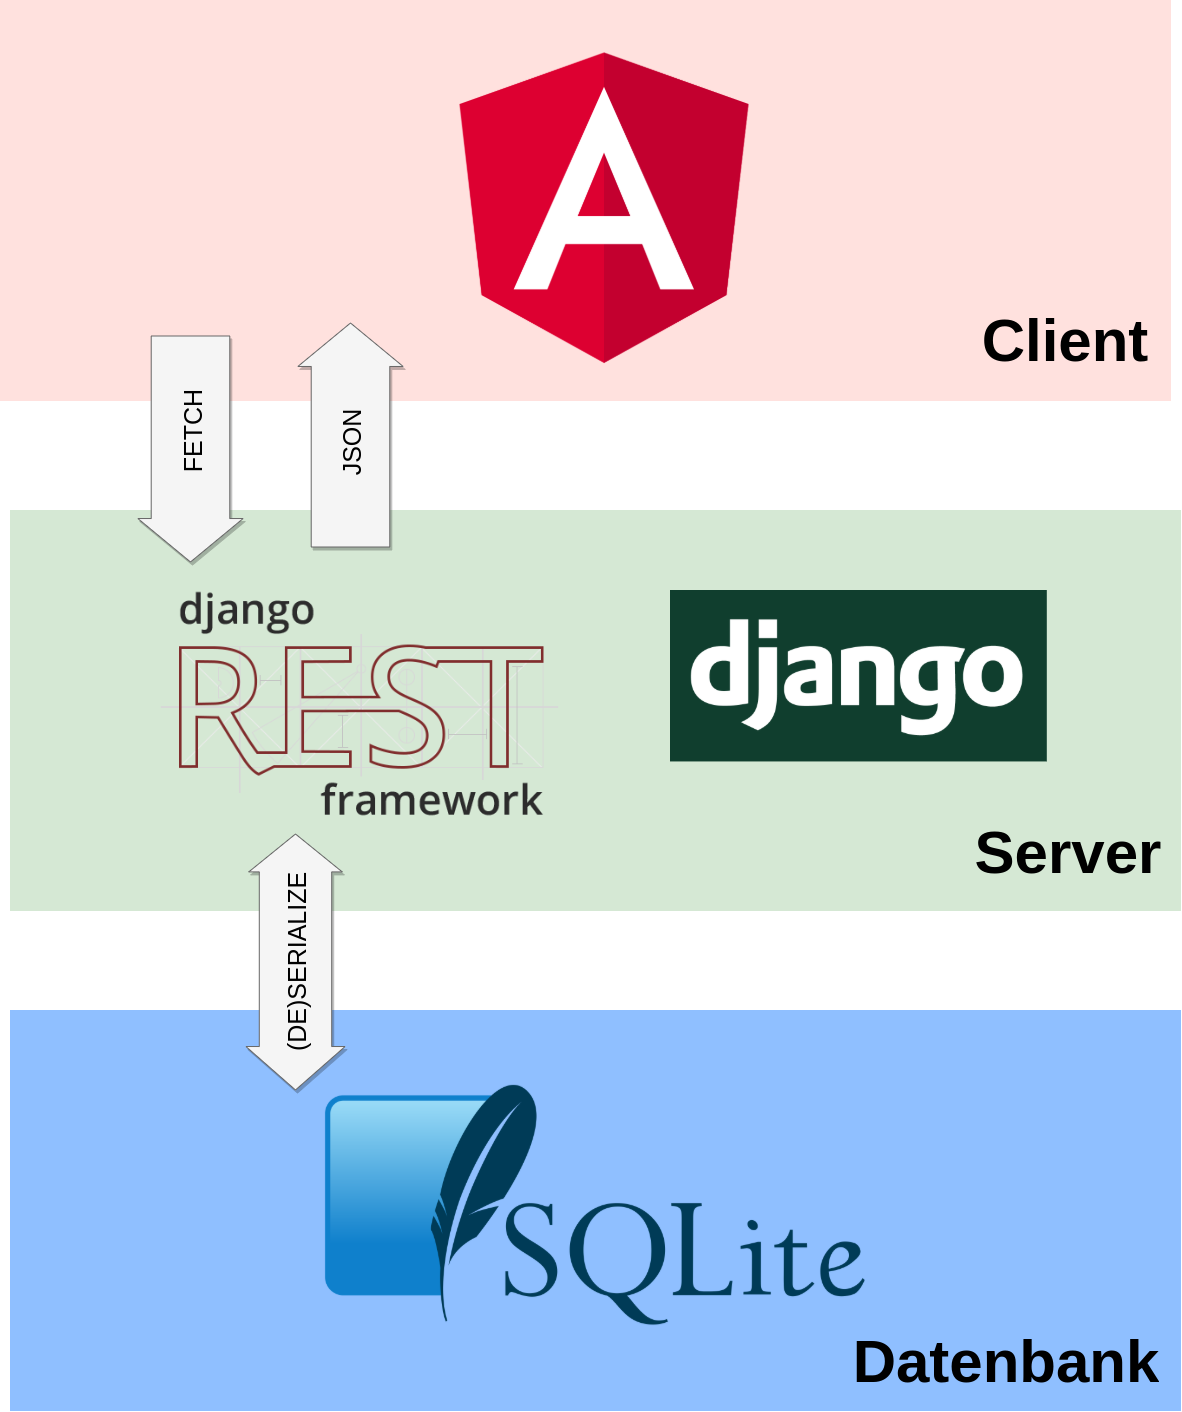
\includegraphics[width=0.7\columnwidth]{./figures/medplanner_stack}
	\caption{Verwendeter Technologie-Stack für MedPlanner}
\end{figure}

\subsection{Architekturentscheidungen}\label{arch-choices}
Wie bereits vorher genannt, wird im Frontend das Framework Angular verwendet. Es stellt einen clientseitigen MVC dar, wodurch eine bessere User Experience mit kürzeren Reaktionszeiten ermöglicht wird. Als Programmiersprache wird TypeScript genutzt, was im Gegensatz zu JavaScript eine Typisierung zulässt und somit logische Typfehler beseitigt. Ein weiterer Grund für diese Entscheidung war die Modularität und Wiederverwendbarkeit. In Angular können Komponenten erstellt und in Module gruppiert werden, die an beliebigen Stellen wiederverwertbar sind. Für einzelne Komponenten ist zudem die Testabdeckung möglich.\\
Für das Backend fiel die Entscheidung auf Django, da es in der Programmiersprache Python implementiert wird, welche das gesamte Team gut beherrscht. Außerdem bietet Django einige Features an wie beispielsweise die Benutzerauthentifizierung oder die Administration der Inhalte über ein Interface.\\
Mithilfe des Django REST Frameworks (DRF) können APIs in Django zur Verfügung gestellt werden, um den Datenaustausch zwischen Angular und Django zu realisieren.\\
Für die Abspeicherung der Daten im Backend wird die relationale Datenbank SQLite verwendet, da die Einrichtung unkompliziert abläuft und die Datenbank trotz geringer Größe viele Funktionalitäten bietet~\cite{sqlite}, die ebenfalls in mächtigeren SQL-Datenbank-Managementsystemen wie MySQL enthalten sind. Im Zusammenhang mit RDBMS und Django ist zu erwähnen, dass das Python-Framework die Realisierung von \textit{n-n-Beziehungen}~\footnote{~Auch bekannt als many-to-many} erlaubt. Dadurch müssen die Entitäten nicht so überarbeitet werden, dass jeweils weitere Tabellen existieren, um one-to-many-Beziehungen zu gewährleisten. Vorteil von Djangos Umsetzung ist, dass in der Datenbank diese Attribute für eine Entität bereits als Liste abgespeichert werden, wodurch größere Anpassungen für die Nutzung und Darstellung im Frontend wegfallen.

\begin{figure}[!h]
	\centering
	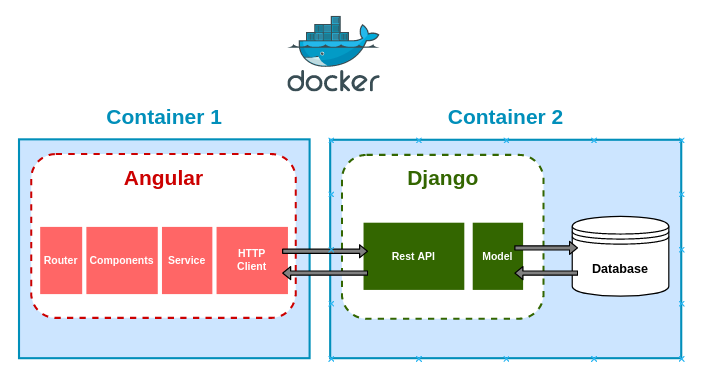
\includegraphics[width=0.9\columnwidth]{./figures/architecture_with_docker}
	\caption{Überblick über das System}
\end{figure}
Für die Realisierung der Web-Anwendung wird eine containerbasierte Architektur unter Verwendung von Docker genutzt. Dabei wird jeweils das Frontend sowie das Backend zusammen mit der Datenbank als Container entwickelt und bereitgestellt. Mittels Docker Compose werden die Container in einem Netzwerk verbunden und können so miteinander kommunizieren. Der Vorteil hierbei ist die schnelle Adaption neuer technologischer Trends: Das System kann ohne unnötigen Aufwand durch eine entsprechende Komposition auch mit anderen Webcontainern eingesetzt werden.
\pagebreak

\subsection{Struktur}\label{structure}

\begin{figure}[!h]
	\centering
	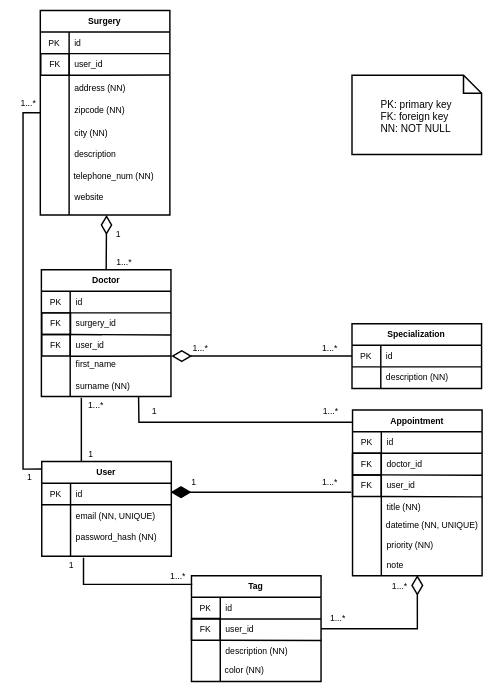
\includegraphics[width=\columnwidth]{./figures/concepts}
	\caption{Datenbankmodell für MedPlanner}
\end{figure}
\textit{Django models} repräsentieren in der Datenbank die unterschiedlichen Entitäten. Dabei wird vom Framework bereits standardmäßig ein User model bereitgestellt, was beispielsweise Attribute wie Vor- und Nachname enthält.~\cite{django-default-user} Da in MedPlanner neben der EMail-Adresse und dem Password zum jetzigen Zeitpunkt keine weiteren Informationen benötigt werden, wurde ein auf die Anforderungen von Medplanner angepasstes User model erstellt.

Für die Identifizierung der Benutzer wird bei MedPlanner die \textit{tokenbasierte Authentifizierung} eingesetzt: So wird bei jeder Registrierung bzw. bei jedem Login ein neues Token für den Benutzer erstellt, womit bestimmte Quellen ohne zusätzliche EMail- oder Passwortinformation abrufbar sind, so beispielsweise auch das Bearbeiten von Terminen. Allgemein werden die Tokens überall dort eingesetzt, wo eine Eingabe von EMail und Passwort nicht dringend benötigt werden.
\pagebreak

\section{Risiken und Probleme}
Im Abschnitt \ref{structure} wurde bereits die Anpassung des User models erwähnt. Standardmäßig wird für das Einfügen eines neuen Benutzers ein Benutzername abgefragt. Durch die Überschreibung des User models wird jedoch für eine Registrierung neben dem Passwort nur eine EMail-Adresse verlangt. Damit dieses Verhalten korrekt übernommen wird, muss zudem eine Überschreibung des Admin models vorgenommen werden, da sonst Konflikte im Backend entstehen. Nach dieser Abänderung ist eine Neuerzeugung der Datenbank erforderlich, um die Aktualisierungen einzupflegen. Aus diesem Grund ist es zwingend ratsam derartige Anpassungen in der Entwicklungsphase vorzunehmen, um größere Migrationsprobleme oder das Risiko für den Verlust von Nutzerdaten zu vermeiden.\\
Die erzeugte SQLite-Datei konnte bei der Versionierung im Versionsverwaltungssystem Git nicht ausgeschlossen werden. Dies hat zur Folge, dass nach jedem Commit, das die Datenbank beeinflusst, Daten verloren gehen können.

Für die Erinnerungsbenachrichtungen per EMail sollte \textit{Django Crontab} genutzt werden. Obwohl die Logik korrekt implementiert war und auch der \textit{Cron Job} aktiv war, konnte die erwartete zeitbasierte Ausführung der Funktionalität mithilfe von Django Crontab nicht realisiert werden. Die Probleme könnten auch auf die Verwendung von Docker zurückgeführt werden.\\
Bezüglich der Testabdeckung im Backend gibt es vereinzelt Einsparungen: Tests für die EMail-Benachrichtungen sind nicht realisiert. Da diese Komponente das allgemeine Systemverhalten nicht stark beeinflusst, wurde das Risiko für den Mangel dieses Testfalls nicht als hoch eingestuft.
Zudem wird das Verhalten für Benutzeraktionen, wie zum Beispiel An- und Abmeldung des Nutzers, nicht mit Tests abgedeckt.



\section{Fazit und Ausblick}
Zum aktuellen Stand bietet MedPlanner ein solides Selbstmanagement-Tool für die Verwaltung von Arztterminen sowie Kontaktinformationen für Arztpraxen. Es ist zudem möglich, direkt eine EMail-Benachrichtigung zu erhalten, sobald ein Patient einen neuen Termin bei MedPlanner erstellt.\\
Für die Zukunft kann diese Benachrichtigungs-Funktionalität so erweitert werden, dass eine Benachrichtigung 24 Stunden vor Terminstart gesendet wird.\\
Außerdem ist denkbar, dass sich Patienten neben geplanten Terminen in Zukunft auch Reminder in einer bestimmten Erinnerungs-Periode setzen können, um an das Vereinbaren eines Termins für Routineuntersuchungen erinnert zu werden.\\
Zusätzlich könnten Termine neben der aktuellen Darstellung auch als Kalender-Einträge visualisiert werden. Somit hätte jeder Patient individuell die Möglichkeit seine bevorzugte Darstellung zu bestimmen.
So wäre es ebenfalls möglich, bei einer EMail-Benachrichtigung eine Eintragung der Termine in eine externe Kalender-App, wie z.B. Google Kalender, bereitzustellen.\\\\
In zukünftigen Versionen könnte MedPlanner auch so ausgebaut werden, dass Patienten neben der Terminverwaltung auch ihre Arztbefunde sicher abspeichern können, um somit alle gesundheitlichen Angelegenheiten kompakt in einer Web-Anwendung strukturieren zu können.\\
Diese Entscheidungen sollten jedoch nicht ausschließlich von den Entwicklern selbst getroffen werden. Mithilfe von Umfragen, ähnlich der Methode des User-Centered-Designs~\footnote{Hierbei werden die späteren Benutzer von Anfang an einbezogen, wodurch Inhalt und Design des Endprodukts maßgeblich von den Bedürfnissen und Erwartungen der Benutzer gesteuert wird.}, können die gewünschten Erweiterungen erfasst werden.

\begin{thebibliography}{00}
\bibitem{sqlite} \url{https://sqlite.org/features.html}
\bibitem{django-default-user} \url{https://docs.djangoproject.com/en/3.2/ref/contrib/auth/#django.contrib.auth.models.User}
\end{thebibliography}
\end{document}
